%%%%%%%%%%%%%%%%%%%%%%%%%%%%%%%%

\documentclass[11pt,a4paper]{article}
\usepackage{times}
\usepackage[utf8]{inputenc}
\usepackage[croatian]{babel}
\usepackage[T1]{fontenc} % Latin Modern

%%%%%%%%%%%%%%%%%%%%%%%%%%%%%%%%


%%%%%%%%%%%%%%%%%%%%%%%%%%%%%%%%
%%%%%%%%  MATEMATICKI PAKETI %%%%%%%%%%%
%%%%%%%%%%%%%%%%%%%%%%%%%%%%%%%%

\usepackage{amsmath}
\usepackage{amsfonts}
\usepackage{amssymb}
\usepackage{esvect}
\usepackage{bm}

%%%%%%%%%%%%%%%%%%%%%%%%%%%%%%%%

%%%%%%%%%%%%%%%%%%%%%%%%%%%%%%%%
%%%%%%%%%% PAKETI ZA SLIKE  %%%%%%%%%%%%
%%%%%%%%%%%%%%%%%%%%%%%%%%%%%%%%

\usepackage{graphicx}
\usepackage{float}
\usepackage[hidelinks]{hyperref}
\usepackage{caption}
\usepackage{subcaption}
\usepackage{booktabs}

%%%%%%%%%%%%%%%%%%%%%%%%%%%%%%%%

%%%%%%%%%%%%%%%%%%%%%%%%%%%%%%%%
%%%%%%%%%    PRORED 1.5   %%%%%%%%%%%%%%
%%%%%%%%%%%%%%%%%%%%%%%%%%%%%%%%

\renewcommand{\baselinestretch}{1.5}

%%%%%%%%%%%%%%%%%%%%%%%%%%%%%%%%


%%%%%%%%%%%%%%%%%%%%%%%%%%%%%%%%
%%%%%%%%%% TABLICA - ANTUN %%%%%%%%%%%%
%%%%%%%%%%%%%%%%%%%%%%%%%%%%%%%%

\usepackage{array}
\usepackage{multirow}
\newcolumntype{C}[1]{>{\centering\let\newline\\\arraybackslash\hspace{0pt}}m{#1}}
\newcolumntype{L}[1]{>{\raggedright\let\newline\\\arraybackslash\hspace{0pt}}m{#1}}
\newcolumntype{R}[1]{>{\raggedleft\let\newline\\\arraybackslash\hspace{0pt}}m{#1}}
\usepackage{ctable}

%%%%%%%%%%%%%%%%%%%%%%%%%%%%%%%%

%%%%%%%%%%%%%%%%%%%%%%%%%%%%%%%%
%%%%%%%%%% TABLICA - MARTINA %%%%%%%%%%%
%%%%%%%%%%%%%%%%%%%%%%%%%%%%%%%%

\makeatletter
\renewcommand*\env@matrix[1][\arraystretch]{%
  \edef\arraystretch{#1}%
  \hskip -\arraycolsep
  \let\@ifnextchar\new@ifnextchar
  \array{*\c@MaxMatrixCols c}}
\makeatother



%%%% LATEX KOD ZA KORISTENJE TABLICE %%%%
%%% PRIMJER %%%

%\setlength\extrarowheight{1pt}
%\begin{table}[h]
%\centering
%\caption{Tablica s prikazom }
%\label{prva}
%\begin{tabular}{|l|c|}
%\hline
%\textbf{txt} &  \\ \hline 
%txt & txt    \\ 
%txt & txt   \\ \hline
%txt & txt    \\ \hline
%\end{tabular}
%\end{table}

%%%%%%%%%%%%%%%%%%%%%%%%%%%%%%%%


%%%%%%%%%%%%%%%%%%%%%%%%%%%%%%%%
%%%%%%% DIO ZA UNOS ISJECAKA KODA %%%%%%%%
%%%%%%%%%%%%%%%%%%%%%%%%%%%%%%%%

\usepackage{listings}
\usepackage{color}
 
\definecolor{codegreen}{rgb}{0,0.6,0}
\definecolor{codegray}{rgb}{0.5,0.5,0.5}
\definecolor{codepurple}{rgb}{0.58,0,0.82}
 
\lstdefinestyle{mystyle}{   
    commentstyle=\color{codegreen},
    keywordstyle=\color{blue},
    numberstyle=\tiny\color{codegray},
    stringstyle=\color{codepurple},
    basicstyle=\footnotesize,
    breakatwhitespace=false,         
    breaklines=true,                 
    captionpos=b,                    
    keepspaces=true,                 
    numbers=left,                    
    numbersep=5pt,                  
    showspaces=false,                
    showstringspaces=false,
    showtabs=false,                  
    tabsize=1
}
 
\lstset{style=mystyle}

%\lstinputlisting[language=Matlab, firstline=1, lastline=4, numbers=left, frame=single, label={lst:prvi}, caption={Diskretizacija sustava korištenjem Matlaba}, captionpos=b]{peti.m} 

%%%%%%%%%%%%%%%%%%%%%%%%%%%%%%%%


%----------------------------
% za uredjenje stranice
\usepackage[left=2.5cm,right=2.5cm,top=2.5cm,bottom=2.5cm]{geometry}
\usepackage{fancyhdr}
\pagestyle{fancy} 
\lhead{\leftmark}
\rhead{\rightmark}
\usepackage{titlesec} %za točku iza broja sectiona
\titleformat{\section}{\huge\bfseries}{\thetitle.\quad}{0em}{}
\titleformat{\subsection}{\LARGE\bfseries}{\thetitle.\quad}{0em}{}
\titleformat{\subsubsection}{\Large\bfseries}{\thetitle.\quad}{0em}{}
\titleformat{\paragraph}
{\normalfont\large\bfseries}{\thetitle.\quad}{1em}{}
\titlespacing*{\paragraph}
{0pt}{3.25ex plus 1ex minus .2ex}{1.5ex plus .2ex}
\setcounter{secnumdepth}{5}

\usepackage{indentfirst} %uvlacenje prvog paragrafa
% primjer pozivanja sectiona
% \section*{UVOD} \pdfbookmark{UVOD}{section:UVOD}

\usepackage{tocloft}
\usepackage{import}
\usepackage{standalone}
\graphicspath{{figures/}} 

\hypersetup{
  colorlinks   = true, %Colours links instead of ugly boxes
  urlcolor     = black, %Colour for external hyperlinks
  linkcolor    = black, %Colour of internal links
  citecolor   = blue %Colour of citations
}

\usepackage{subcaption}
\usepackage{lscape}
\begin{document}

U sklopu ovog poglavlja izveden je nelinearni matematički model letjelice koji opisuje njezinu rotaciju i translaciju. Na temelju tog modela obavlja se njegova linearizacija u svrhu dobivanja prijenosne funkcije sustava koja se potom koristi za upravljanje. 

\medskip

\subsection{Nelinearni dinamički model letjelice s pokretnim masama}

Koordinatni sustav letjelice prikazan je slikom \ref{fig:mod}. Svi vektori korišteni za opis ovog sustava, uz iznimku sile gravitacije, izraženi su u lokalnom mobilnom koordinatnom sustavu letjelice označenom s $L_{0}$. Vektor sile gravitacije prikladno je izražen u globalnom nepomičnom koordinatnom sustavu $L_{I}$. $L_{CoG}$ označava koordinatni sustav vezan za centar mase letjelice te je on usklađen s $L_{0}$ koordinatnim sustavom.


\begin{figure}[H]
	\centering
	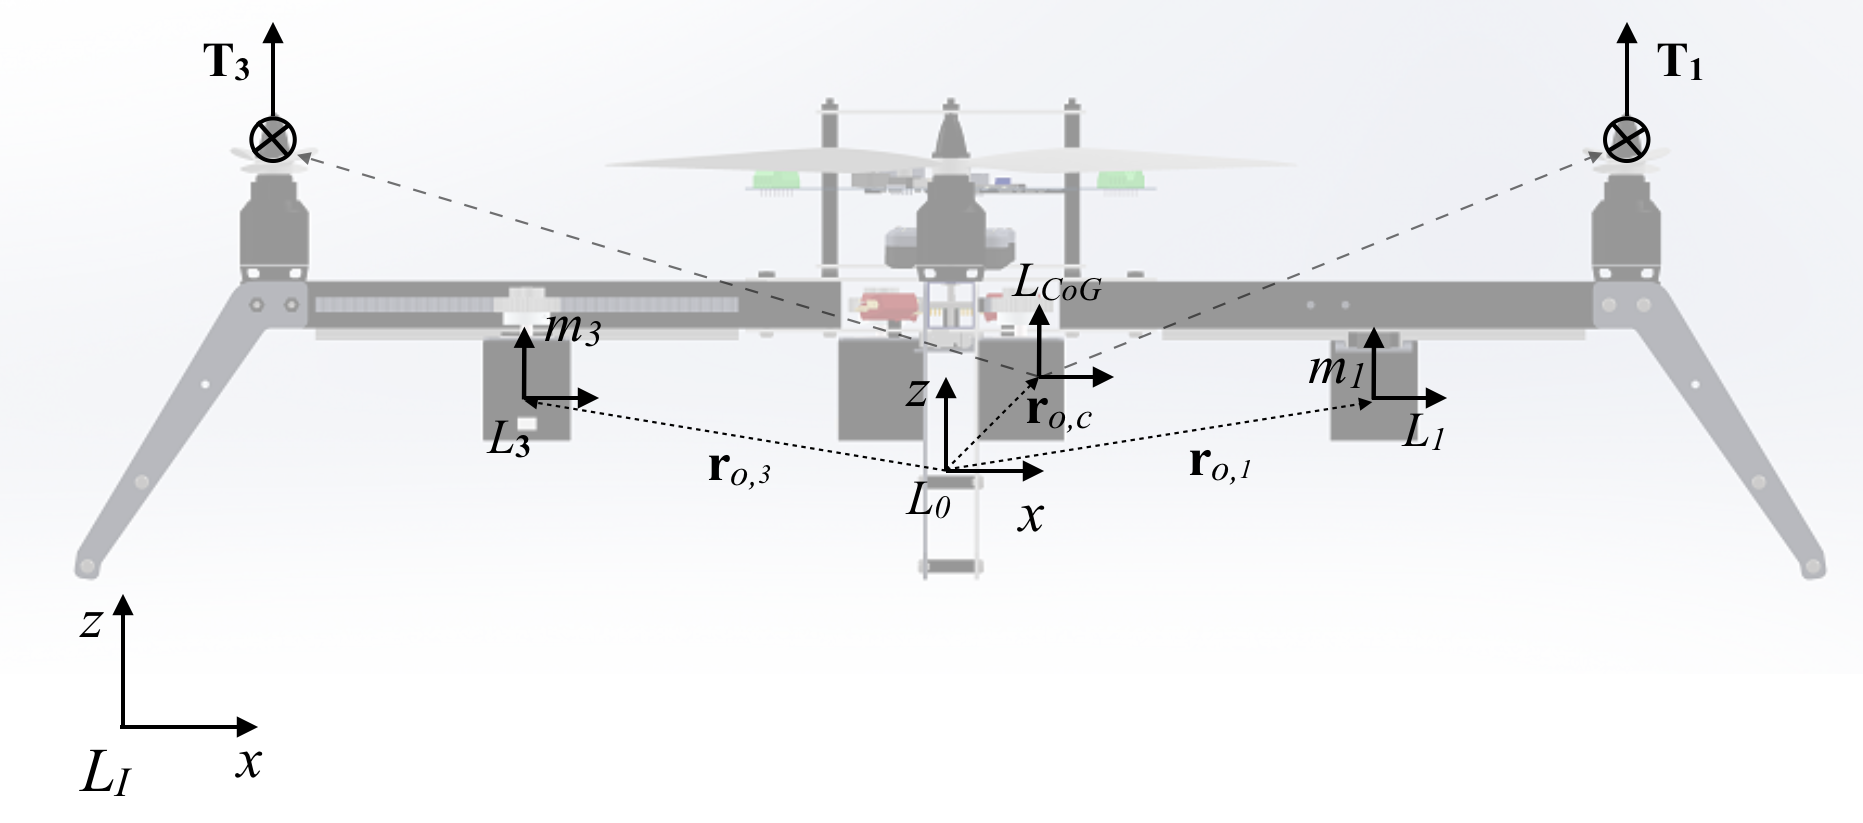
\includegraphics[scale=0.23]{model}
	\caption{Koordinatni sustav letjelice \cite{haus1}}
	\label{fig:mod}
\end{figure}

Matematičko modeliranje započinje se standardnim zapisom formule za proizvoljni vektor promjenjive duljine izražen u lokalnom mobilnom koordinatnom susavu letjelice ($L_{0}$):

\begin{equation}
\frac{d^{\omega}}{dt}({r}_{0}) =  {\dot{r}}_{0} + {\omega} \times {r}_{0} 
\label{eq:r0}
\end{equation}

gdje $\boldsymbol{\dot{r}_{0}}$ označa vektor stope promjene u $L_{0}$ koordinatnom sustavu, dok $\omega$  označava kutnu brzinu gibanja letjelice, odnosno kutnu brzinu gibanja $L_{0}$ koordinatnog sustava. 

\medskip

Centar mase letjelice promatran iz lokalnog koordinatnog sustava dan je sljedećim izrazom:

\begin{equation}
 {r}_{0,c} = \frac{ {m}_{b} {r}_{0,b} + \sum_{i=1}^{4}{m}_{i} {r}_{0,i}}{{m}_{b} + \sum_{i=1}^{4} {m}_{i}} = \frac{\sum_{i=1}^{4} {m}_{i} {r}_{0,i}}{ {M}}
\label{eq:r0c}
\end{equation}

\begin{equation}
 {v_{c} = v_{0} + v_{0,c} + \omega \times r_{0,c}}
\label{eq:vc}
\end{equation}

\begin{equation}
 {v_{0,c} = \frac{\sum_{i=1}^{4}m_{i}\dot{r}_{0,i}}{M}}
\label{eq:v0c}
\end{equation}

\begin{equation}
 {v_{i} = v_{0} + v_{0,i} + \omega \times r_{0,i}}
\label{eq:vi}
\end{equation}

\begin{equation}
 {v_{i} = v_{c} + v_{0,i} - v_{0,c} + \omega \times r_{c,i}}
\label{eq:vi2}
\end{equation}

\begin{equation}
 {L_{i} = m_{i} \cdot v_{i}}
\label{eq:Li}
\end{equation}

\begin{equation}
 {\frac{d^{\omega}}{dt} L_{i} = \sum_{k=1}^{3}f_{ik}}
\label{eq:Lidot}
\end{equation}

\begin{equation}
f_{i1}  =K_{m}T_{r}U_{i}\left(\sin\left(\frac{\pi}{2}i\right) \bm{\hat{i}} - \cos\left( \frac{\pi}{2}i\right) \bm{\hat{j}}\right), i \in \{1,2,3,4\}
\label{eq:fi1}
\end{equation}

\begin{equation}
f_{i2} = -m_{i}\cdot g \bm{\hat{K}}
\label{eq:fi2}
\end{equation}

\begin{equation}
f_{i3} = -c_{d} \cdot v_{0,i}
\label{eq:fi3}
\end{equation}


\begin{equation}
\frac{d^{\omega}}{dt}v_{0,i} = \frac{1}{m_{i}}\left(\sum_{k=1}^{3}f_{ik}\right) - \frac{d^{\omega}}{dt} \left( v_{0} + \omega \times r_{0,i} \right) 
\label{eq:voidot}
\end{equation}



\begin{equation}
L_{s} = L_{b} + \sum_{i=1}^{4}L_{i}
\label{eq:Ls}
\end{equation}


\begin{equation}
L_{s} = M \cdot (v_{0} + \omega \times r_{0,c}) + \sum_{i=1}^{4}m_{i}c_{0,i} = M \cdot (v_{0} + \omega \times r_{0,c}) + \sum_{i=1}^{4}L_{0,i}
\label{eq:Ls2}
\end{equation}


\begin{equation}
\frac{d^{\omega}}{dt} v_{0} = \frac{1}{M} \left( \sum_{j=1}^{4} F_{rj} + F_{g} - \frac{d^{\omega}}{dt} \sum_{i=1}^{4}L_{0,i}  \right) - \frac{d^{\omega}}{dt} (\omega \times r_{0,c})
\label{eq:v0dot}
\end{equation}


\begin{equation}
F_{rj} = b_{f}\Omega_{j}^{2} \bm{\hat{k}}
\label{eq:Frj}
\end{equation}

\begin{equation}
T_{r}\dot{\Omega}_{j} + \Omega_{j} = \Omega_{r,j}
\label{eq:omega_rj}
\end{equation}

\begin{equation}
F_{g} = -Mg \bm{\hat{K}}
\label{eq:Fg}
\end{equation}

\begin{equation}
H_{s} = H_{b} + \sum_{i=1}^{4}H_{i}
\label{eq:Hs}
\end{equation}

\begin{equation}
H_{b} = \int_{k} r_{c,k} \times (v_{k}dm_{k}) = \int_{k} r_{c,k} \times (v_{c} + v_{0,k} - v_{0,c} + \omega \times r_{c,k})dm_{k}
\label{eq:Hb}
\end{equation}

\begin{equation}
H_{i} = \int_{ji} r_{c,ji} \times (v_{ji}dm_{ji}) = \int_{ji} r_{c,ji} \times (v_{c} + v_{0,i} - v_{0,c} + \omega \times r_{c,ji})dm_{ji}
\label{eq:Hi}
\end{equation}

\begin{equation}
H_{s} = I_{s}^{c}\omega + \sum_{i=1}^{4}r_{c,i} \times L_{0,i}
\label{eq:Hs2}
\end{equation}

\begin{equation}
I_{s}^{c} = I_{b}^{c} + \sum_{i=1}^{4}I_{i}^{c}
\label{eq:Ics}
\end{equation}

\begin{equation}
I_{i}^{c} = I_{i} + m_{i} \left(  r_{ci,}^{T} \cdot r_{c,i}E_{3} - r_{c,i}\cdot r_{c,i}^{T} \right)
\label{eq:Iic}
\end{equation}

\begin{equation}
\frac{d^{\omega}}{dt} \left( I_{s}^{c} \omega + \sum_{i=1}^{4} r_{c,i}\times L_{0,i}  \right) = \sum_{j=1}^{4}(M_{fi} + M_{dj}) + M_{g}
\label{eq:dtM}
\end{equation}

\begin{equation}
M_{fj} = r_{d,rj} \times F_{rj} = (r_{c,0} + r_{0,rj}) \times F_{rj}
\label{eq:Mfj}
\end{equation}

\begin{equation}
M_{dj} = \zeta_{j}b_{m}b_{f}\Omega_{j}^{2} \bm{\hat{k}}
\label{eq:Mdj}
\end{equation}


\begin{equation}
M_{g} = r_{c,b} \times (-m_{b}g \bm{\hat{K}}) + \sum_{i=1}^{4} \times (-m_{i}g \bm{\hat{K}})
\label{eq:Mg}
\end{equation}

\end{document}